\chapter{評估與結果}

\section{結果呈現}

\subsection{Repository}
由於協同需求,本組採用Github倉儲作為程式碼交流、圖檔存放、網站維護及架設的環境。
組員透過fork倉儲,編輯後再提出pull request進行merge,即可升級倉儲。

\begin{figure}[h]
    \centering
    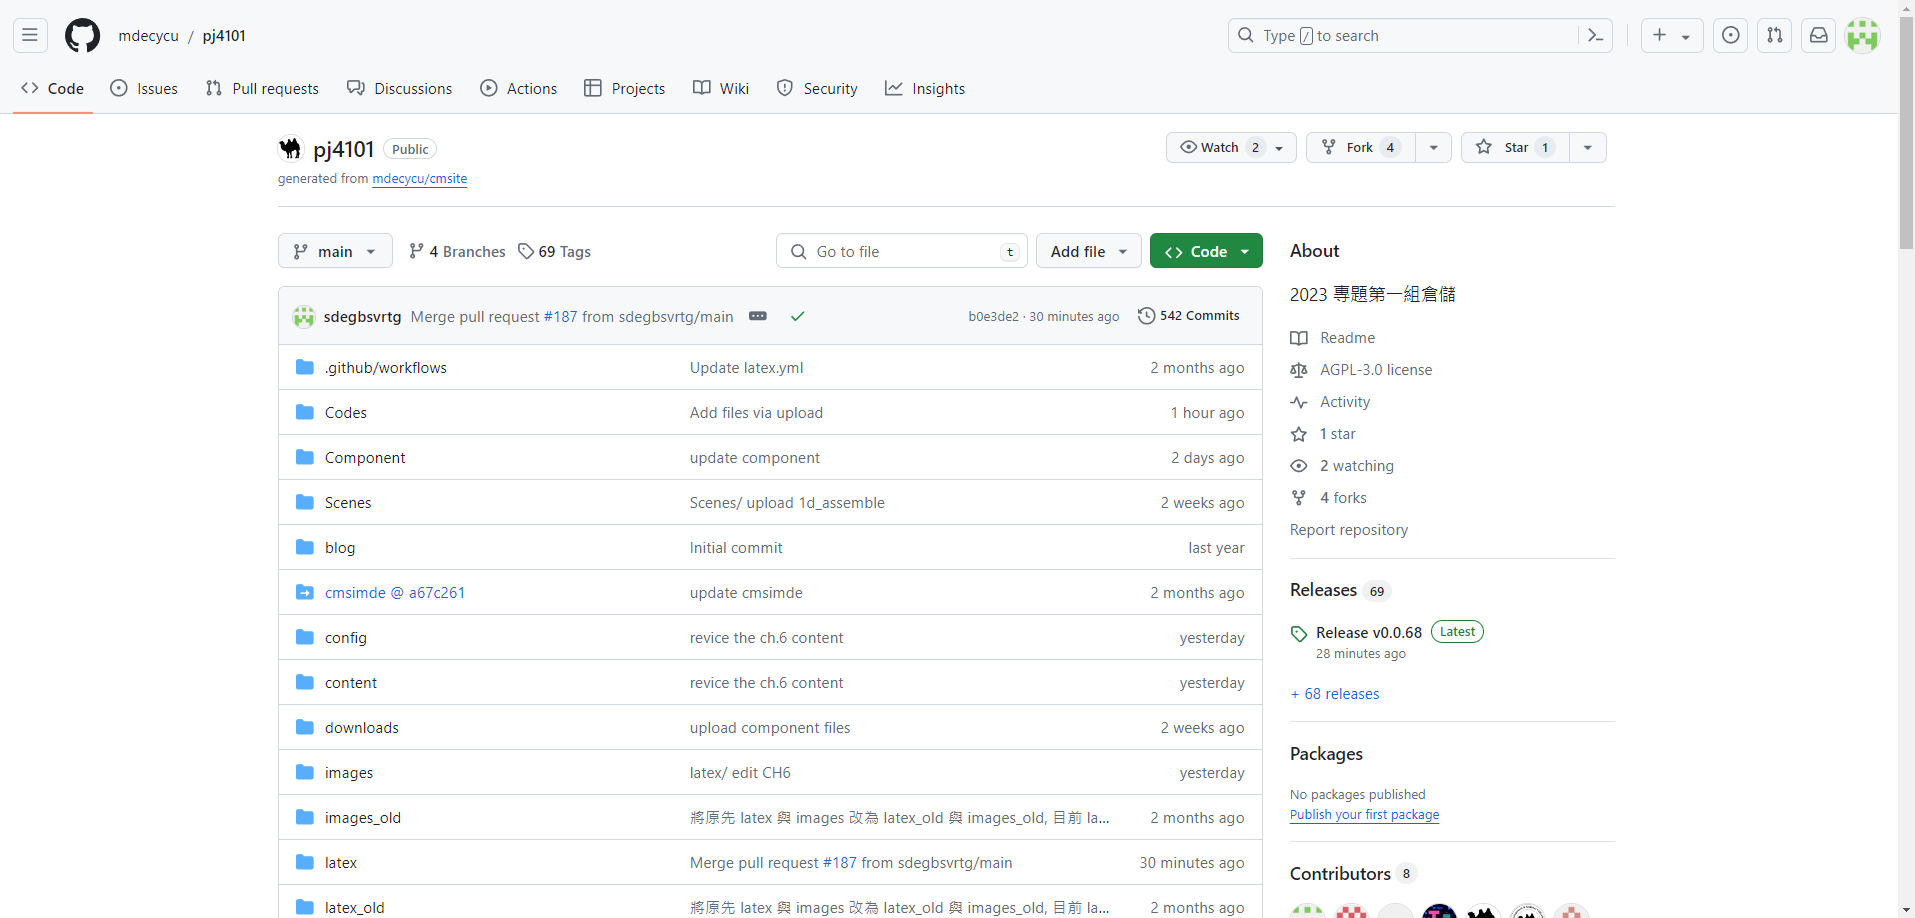
\includegraphics[width=0.8\textwidth]{repo}
    \caption{本組專題倉儲}
\end{figure}

在倉儲內可查看組員的更新紀錄,並且倉儲內保留著每一版次的資料,可以隨時查看先前的檔案。

\begin{figure}[h]
    \centering
    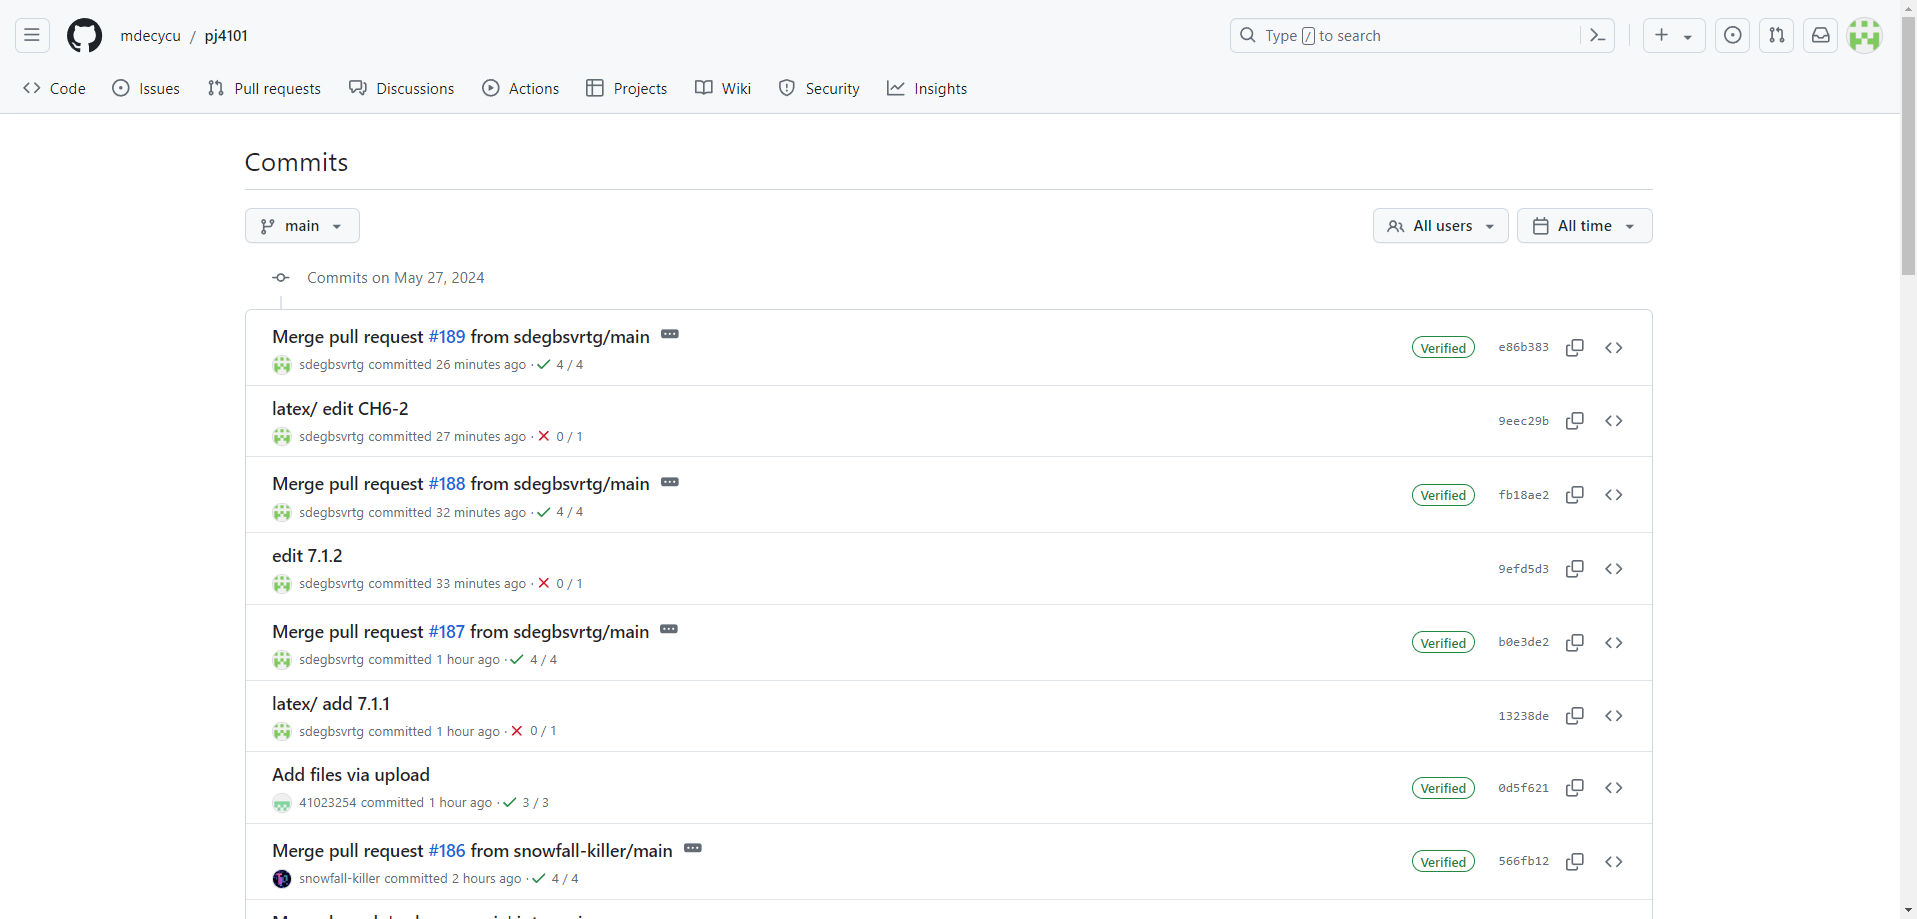
\includegraphics[width=0.8\textwidth]{7rep_v}
    \caption{倉儲更新紀錄}
\end{figure}

在倉儲內也可透過設定.yml檔,使用LaTeX生成俱有版次的PDF報告。

\begin{figure}[h]
    \centering
    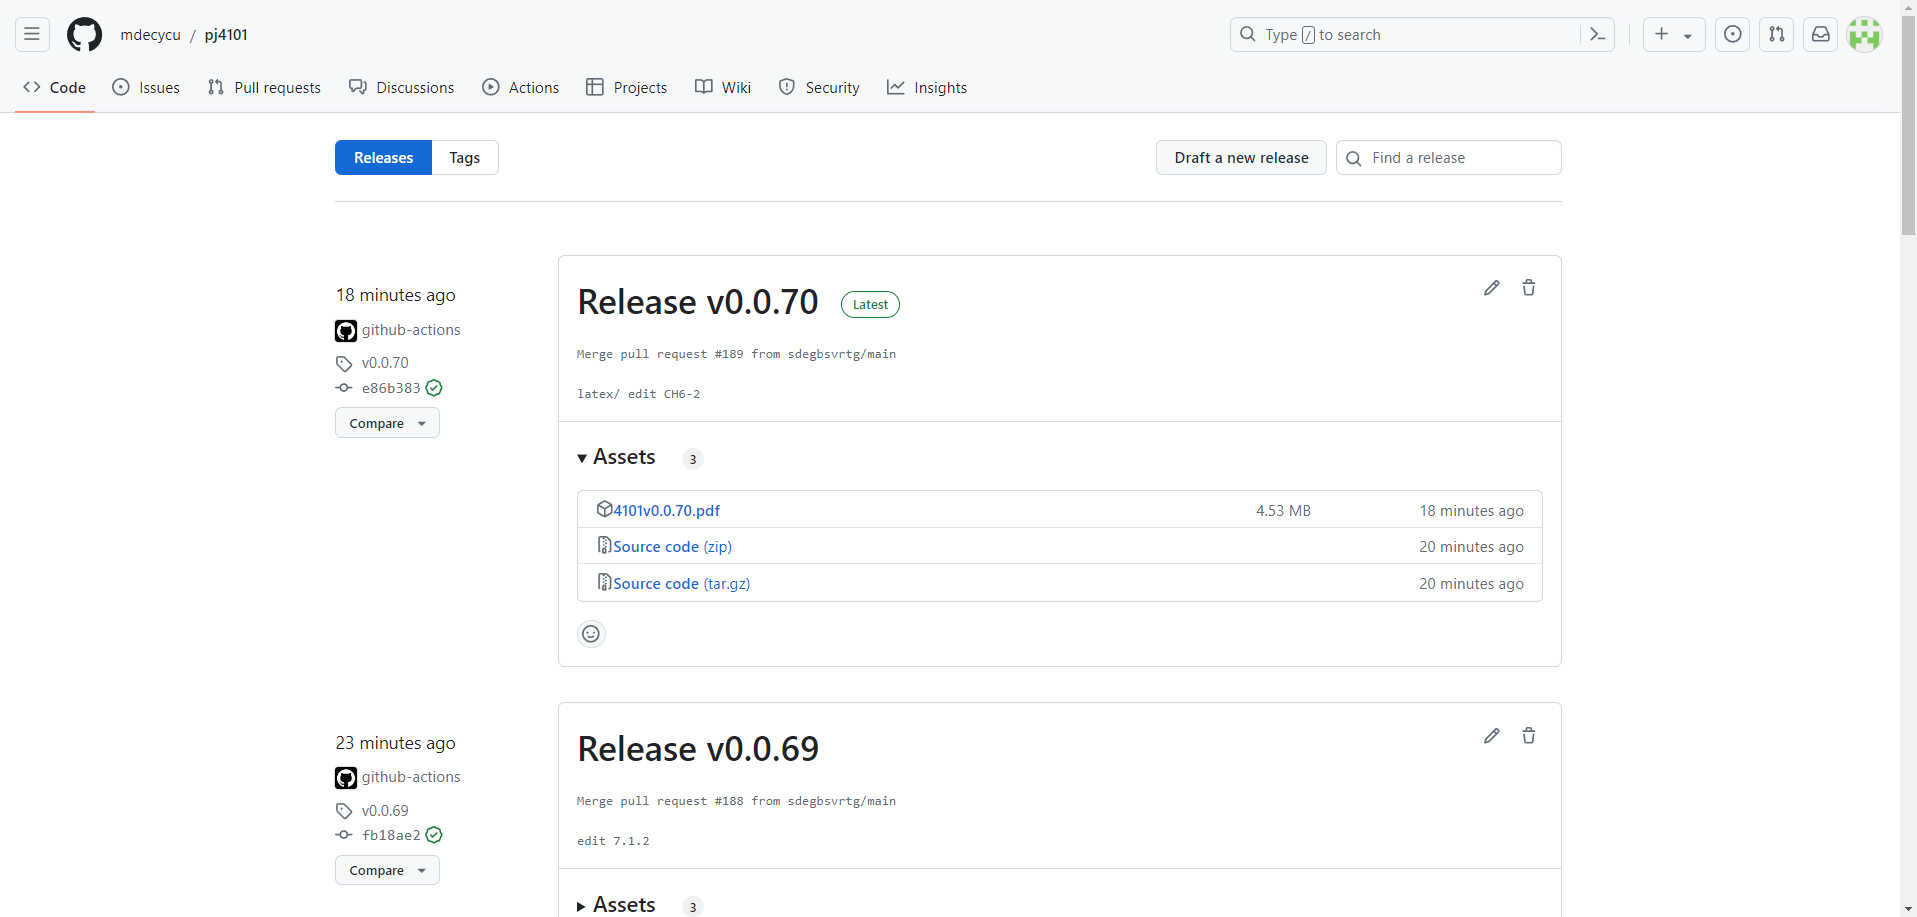
\includegraphics[width=0.8\textwidth]{7pdf_v}
    \caption{PDF報告釋出版次}
\end{figure}

\subsection{Github Page}
本組專題成果網頁係藉由藉由本組指導教授嚴家銘教授所開發的cmsimde子模組進行維護。\\

\begin{figure}[h]
    \centering
    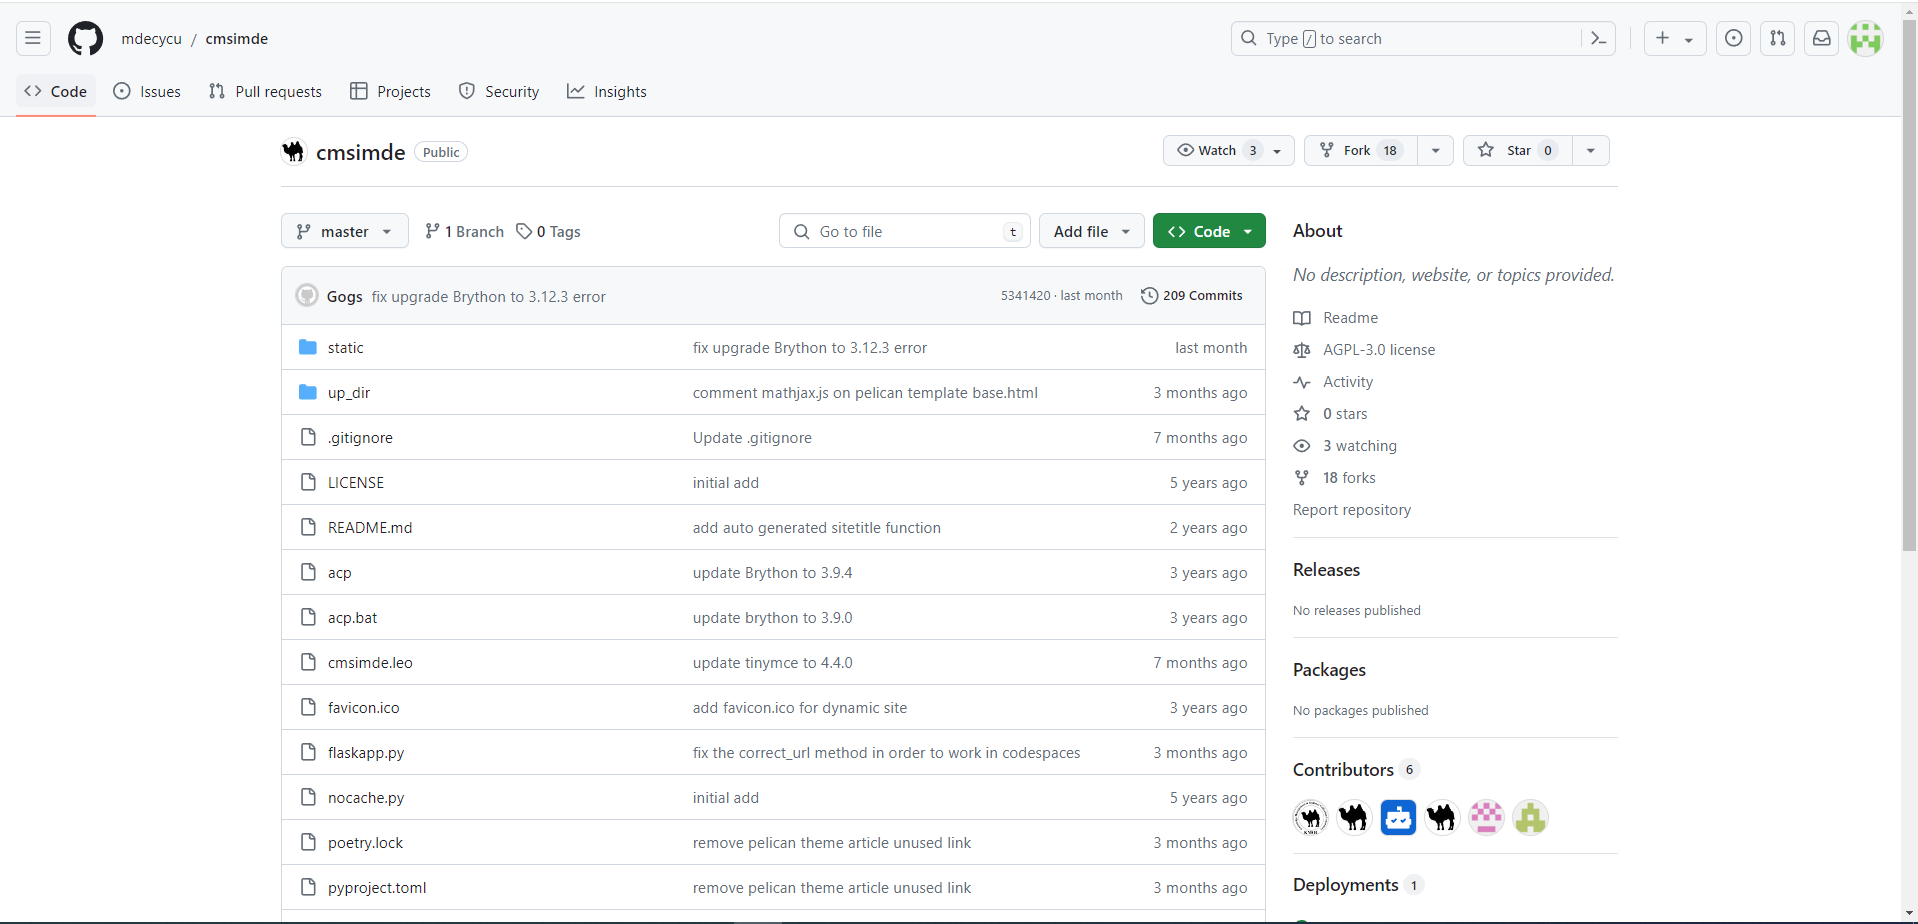
\includegraphics[width=0.8\textwidth]{cmsimde}
    \caption{cmsimde}
\end{figure}

組員只要在可攜環境的近端倉內使用終端機執行cms.bat,就會以python運行cmsimde資料夾中的wsgi.py,
接著就會透過flaskapp.py等檔案啟動近端的動態網頁。
組員即可透過瀏覽器編輯動態網頁,編輯完成後亦可透過編輯器內的選項將動態網頁轉換為靜態,並推送至Github倉儲中,由遠端倉儲生成網頁,
網址為\url{https://mde.tw/pj4101}。\\

\begin{figure}[h]
    \centering
    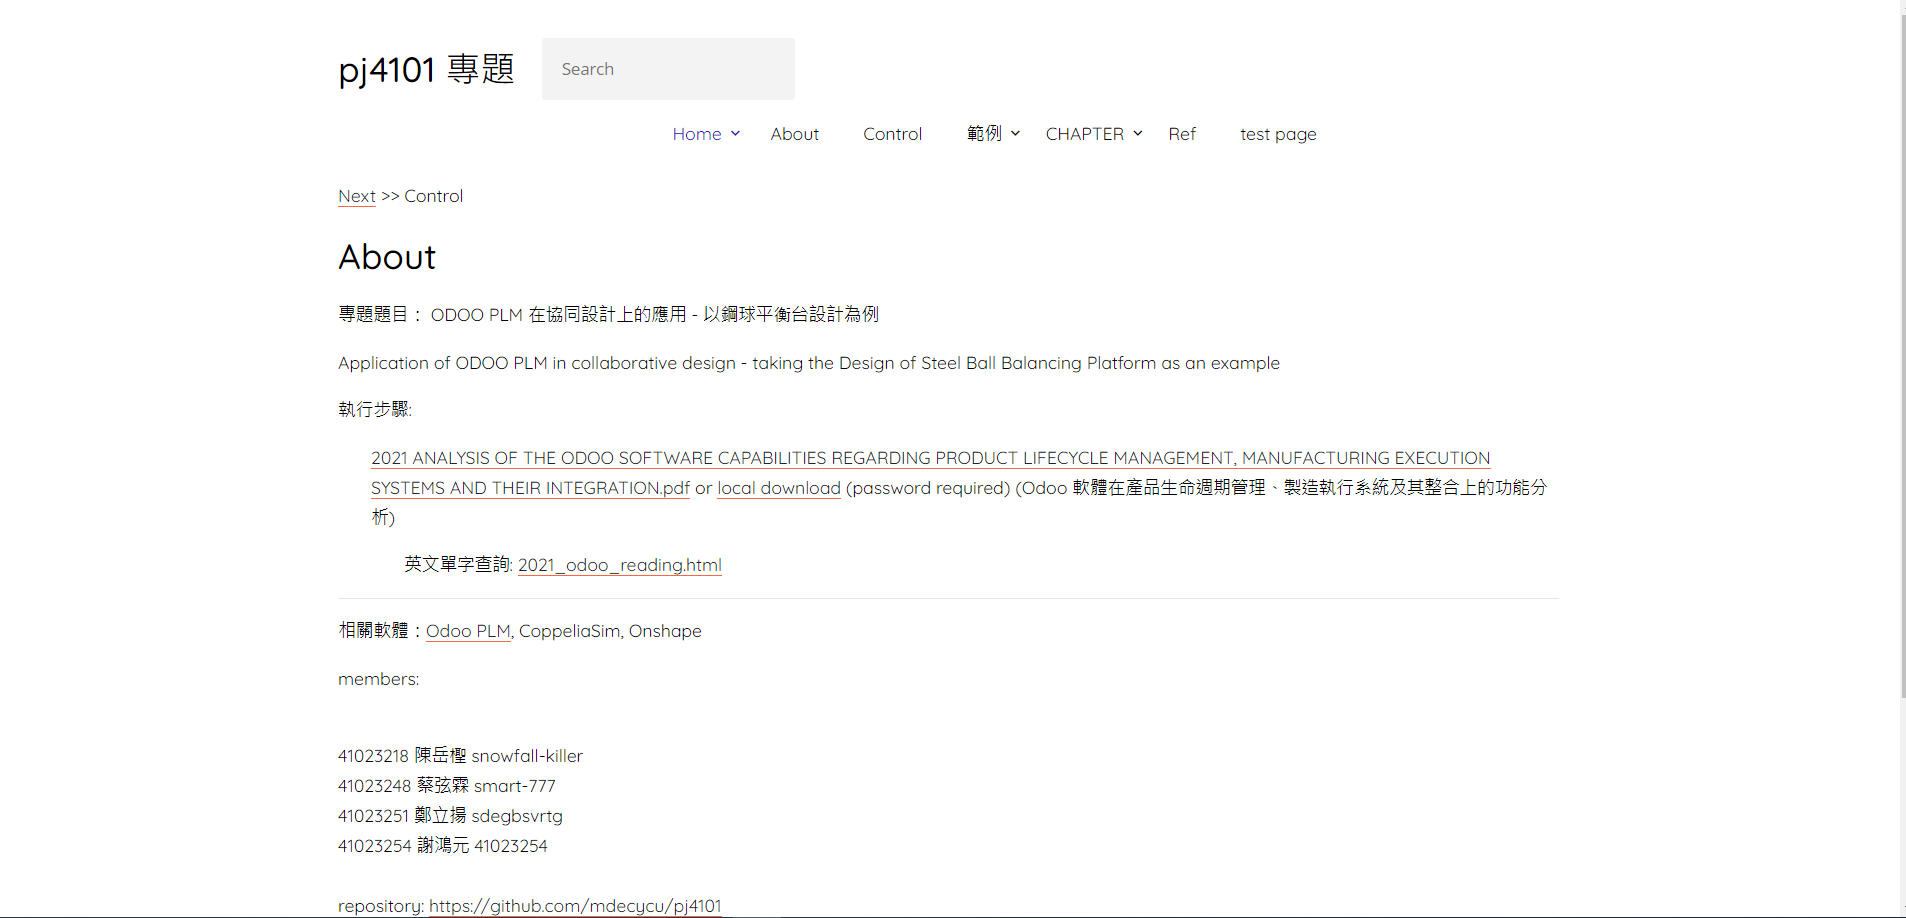
\includegraphics[width=0.8\textwidth]{mdepj4101}
    \caption{本組專題網頁}
\end{figure}

在此環境之下,本組組員能非常輕鬆的協同對網頁進行維護。\\




\subsection{PID控制}
在經過計算後,我們得到了KP=38.5,KI=5,KD=31.5。但由於系統誤差,導致系統平衡較慢,因此我們進行手動調整得到控制參數為KP=38.2,KI=5,KD=31.6。



\section{結果分析}

\subsection{LaTeX-PDF報告}
因為使用latex製作PDF報告,組員們可以同時編輯報告的不同章節,在近端透過可攜環境中的miktex,可以生成並預覽PDF報告,大大提升了協同的效率。也因為LaTeX對數學公式的支援,在製作報告時我們只要輸入指令,
就能產生各種數學公式符號,不需要逐一點選。在我們的專題環境中只要透過github更新.tex檔案,就會自動生成新版本的PDF報告,相當方便。
\subsection{}
\subsection{}

\section{討論}
\subsection{}
\subsection{}
\subsection{}